\documentclass[letterpaper,12pt]{article}
\usepackage{tabularx} % extra features for tabular environment
\usepackage{amsmath}  % improve math presentation
\usepackage{float}
\usepackage{pdfpages}

\usepackage{multicol}
\usepackage{graphicx} % takes care of graphic including machinery
\graphicspath{ {./figures/} }
%\usepackage[margin=1in,letterpaper]{geometry} % decreases margins
%\usepackage{cite} % takes care of citations
\usepackage[final]{hyperref} % adds hyper links inside the generated pdf file
\hypersetup{
	colorlinks=true,       % false: boxed links; true: colored links
	linkcolor=blue,        % color of internal links
	citecolor=blue,        % color of links to bibliography
	filecolor=magenta,     % color of file links
	urlcolor =blue         
}
\usepackage[margin = 1in,headsep=0.5cm,headheight=2cm,letterpaper]{geometry} 

\usepackage{fancyhdr}
\pagestyle{fancy}
\lhead{Student 1 : Ahmet Akman 2442366 \\ Student 2: Yusuf Toprak Yıldıran 2444149 \\ Assistant: Onur Selim Kılıç}
\rhead{Date: \today \\ Group: Wednesday Morning - 5} 
%\cfoot{center of the footer!}
\renewcommand{\headrulewidth}{0.1pt}



\begin{document}
\thispagestyle{empty}

\title{Spring 2022 EE214 Experiment 4  \protect\\ Impedance Measurement and Complex Power}
\author{Ahmet Akman 2442366 \protect\\ Yusuf Toprak Yıldıran 2444149 \protect\\ Assistant: Onur Selim Kılıç}
\date{\today}
\maketitle
\tableofcontents
%\begin{abstract}
%abstract
%\end{abstract}
\section{Introduction}
\section{Experimental Results and Discussion}
The results of the experiment are discussed in the following steps.
%
\subsection{Step 1}
\begin{figure}[H]
    \centering
    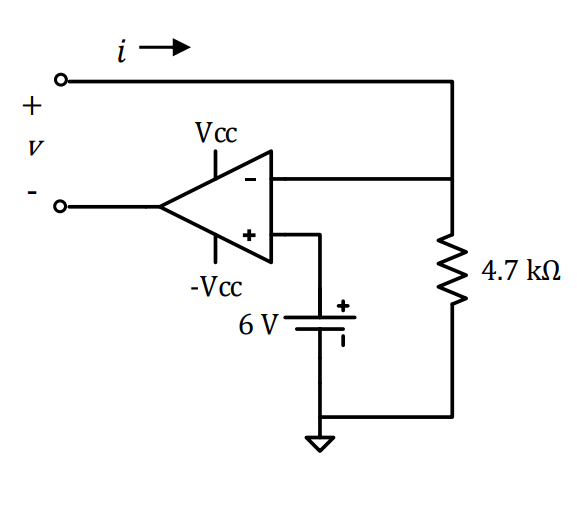
\includegraphics[width = 0.75\textwidth]{1SCH.png}
    \caption{Circuit schematic for the step 1}
\end{figure} 
    
\subsubsection{a.}

\subsubsection{b.}

\subsubsection{c.}

\subsubsection{d.}

\begin{table}[H]
    \begin{center}
        \caption{Power Measurements}
        \vspace{2mm}
        \begin{tabular}{||c | c | c | c | c | c | c ||} 
            \hline
            Part & \(V_{in}\)\newline (Vrms) & \(V_{line}\)\newline (Vrms) & \(V_{Load}\) \newline (Vrms) &\(i_{Load}\)\newline (mArms) & \(\phi_{Load}\)\newline(degree) &\(\phi_{in}\)\newline(degree)  \\ [0.5ex] 
            \hline\hline
            a. & &  & & & &   \\ 
            \hline
            b. & &  & & & &    \\
            \hline
            c. & &  & & & &   \\ [1ex] 
            \hline
        \end{tabular}
\end{center}
\end{table}


\begin{table}[H]
    \begin{center}
        \caption{Power Calcuations}
        \vspace{2mm}
        \begin{tabular}{||c | c | c | c | c | c ||} 
            \hline
            Part & \(P_{in}\)\newline (mW) & \(P_{line}\)\newline (mW) & \(P_{Load}\) \newline (mW) &\(Q_{Load}\)\newline (mVAR) & \(|S|_{Load}\)\newline(mVA)   \\ [0.5ex] 
            \hline\hline
            a. & &  & & &    \\ 
            \hline
            b. & &  & & &     \\
            \hline
            c. & &  & & &    \\ [1ex] 
            \hline
        \end{tabular}
\end{center}
\end{table}




\begin{table}[H]
  \begin{center}
    \caption{Load Parameters}
    \vspace{2mm}
 \begin{tabular}{||lll|lll|lll||}
    \hline
    \multicolumn{3}{|l|}{Part a. (Load)}                            & \multicolumn{3}{l|}{Part b. Load}                            & \multicolumn{3}{l|}{Part c. Load}                            \\ \hline
    \multicolumn{1}{|l|}{pf} & \multicolumn{1}{l|}{lead/lag} & eff \(\%\) & \multicolumn{1}{l|}{pf} & \multicolumn{1}{l|}{lead/lag} &eff \(\%\)  & \multicolumn{1}{l|}{pf} & \multicolumn{1}{l|}{lead/lag} &eff \(\%\)  \\ \hline
    \multicolumn{1}{|l|}{} & \multicolumn{1}{l|}{} &  & \multicolumn{1}{l|}{} & \multicolumn{1}{l|}{} &  & \multicolumn{1}{l|}{} & \multicolumn{1}{l|}{} &  \\ \hline
    \end{tabular}
\end{center}

\end{table}
\subsection{Step 2}
\begin{figure}[H]
    \centering
    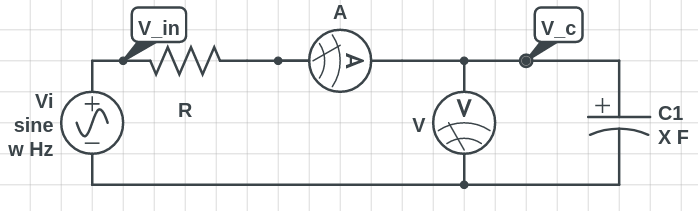
\includegraphics[width = 0.75\textwidth]{2SCH.png}
    \caption{Circuit schematic for the step 2}
\end{figure} 
    
\subsection{Step 3}
\begin{figure}[H]
    \centering
    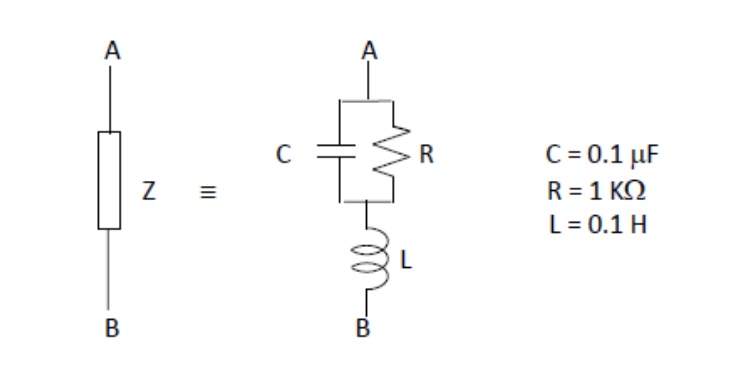
\includegraphics[width = 0.75\textwidth]{3SCH.png}
    \caption{Circuit schematic for the step 3}
\end{figure} 

\begin{figure}[H]
    \centering
    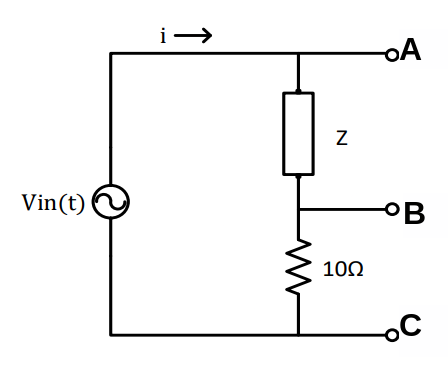
\includegraphics[width = 0.75\textwidth]{3_1SCH.png}
    \caption{Outside circuit schematic for the step 3}
\end{figure} 

\section{Conclusion}


\section*{Appendix A}
\begin{itemize}
    \item PreLab Preparation 3 hours
    \item Experimental Work 2  hours
    \item Report Writing 8 hours
\end{itemize}

\end{document}

%%%%%%%%%%%%%%%%%%%%%%   EXAMPLE TABLE   %%%%%%%%%%%%%%%%%%%%%%%%%%%%%%%%
\begin{table}[H]
\begin{center}
    \caption{Resistance reading by color code convention.}
    \vspace{2mm}
    \begin{tabular}{||c | c | c||} 
        \hline
        Color Order & Value & Tolerance \\ [0.5ex] 
        \hline\hline
        Brown / Black / Red / Gold & 1k\( \Omega \) & \( \% \) 5  \\ 
        \hline
        Yellow / Violet / Red / Gold & 4.7k\( \Omega \) & \( \% \) 5   \\
        \hline
        Brown / Grey / Orange / Gold & 18k\( \Omega \) & \( \% \) 5  \\ [1ex] 
        \hline
    \end{tabular}
\end{center}
\end{table}


%%%%%%%%%%%%%%%%%%%%%%   EXAMPLE IMAGE   %%%%%%%%%%%%%%%%%%%%%%%%%%%%%%%%
\begin{figure}[H]
\centering
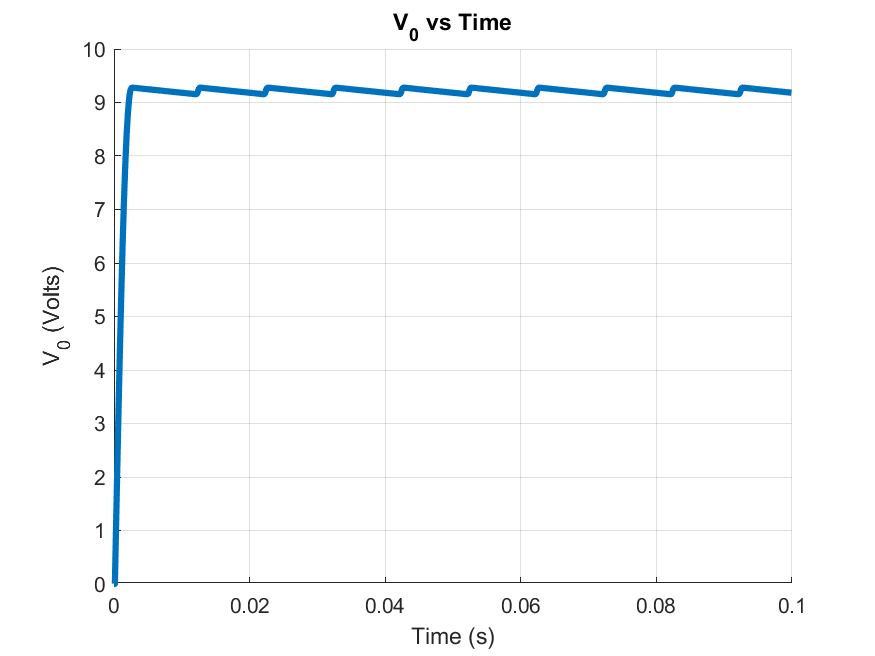
\includegraphics[width = 0.75\textwidth]{5.png}
\caption{Circuit schematic for the step 5}
\end{figure} 

%%%%%%%%%%%%%%%%%%%%%%   EXAMPLE IMAGE FROM PDF   %%%%%%%%%%%%%%%%%%%%%%%%%%%%%%%%
\begin{figure}[H] \centering{
	\includegraphics[scale=0.25]{2a_plot.pdf}}
	\caption{Experiment 2}
\end{figure}
%%%%%%%%%%%%%%%% Deneme Push